\section{Modelo de Mezcla Gaussiana} \label{sec_GMM}

Do Chuong y Batzoglou nos indican, en su artículo \textit{What is the expectation maximization algorithm?} [\ref{ChuongBatzoglou}], que el algoritmo de maximización de la esperanza (EM) es una generalización natural de la estimación por máxima verosimilitud. Ésto para el caso en donde se tiene información incompleta.

Los parámetros iniciales se toman de los datos con ello se obtienen unos parámetros finales que se convierten en los parámetros de la siguiente iteración. Así sucesivamente.


\begin{figure}[H]
\centering
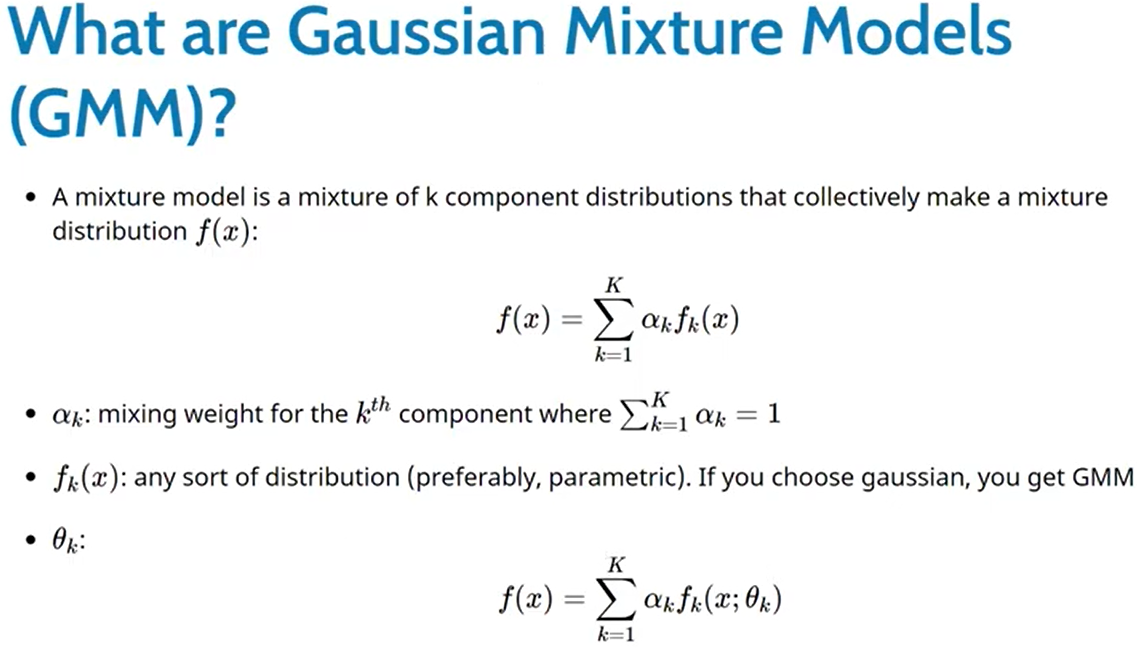
\includegraphics[scale = 0.5]{GMM_1} %width=\textwidth
\caption{\textit{GMM 1}}
\end{figure}

\begin{figure}[H]
\centering
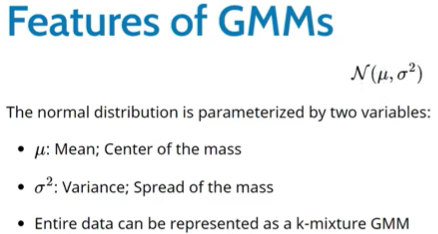
\includegraphics[scale = 0.5]{GMM_2} %width=\textwidth
\caption{\textit{GMM 2}}
\end{figure}

\begin{figure}[H]
\centering
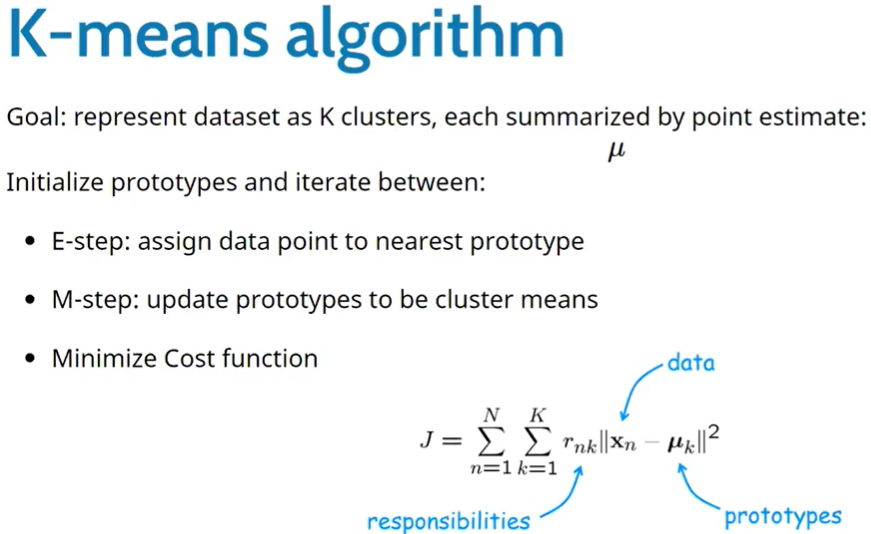
\includegraphics[scale = 0.5]{GMM_3} %width=\textwidth
\caption{\textit{GMM 3}}
\end{figure}

\begin{figure}[H]
\centering
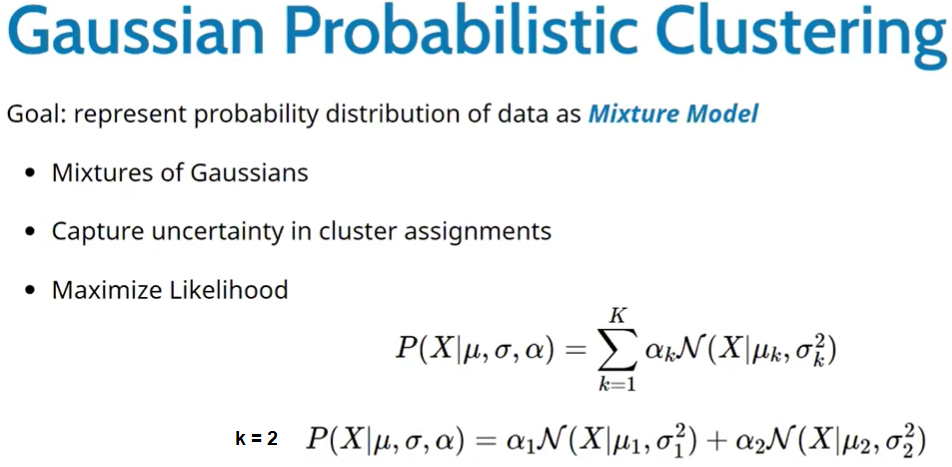
\includegraphics[scale = 0.5]{GMM_4} %width=\textwidth
\caption{\textit{GMM 4}}
\end{figure}

\begin{figure}[H]
\centering
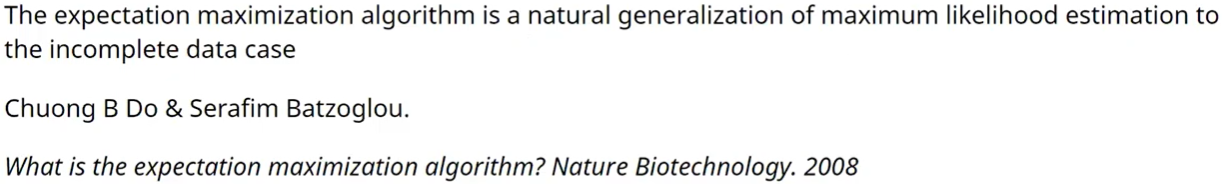
\includegraphics[scale = 0.5]{GMM_5} %width=\textwidth
\caption{\textit{GMM 5}}
\end{figure}

\begin{figure}[H]
\centering
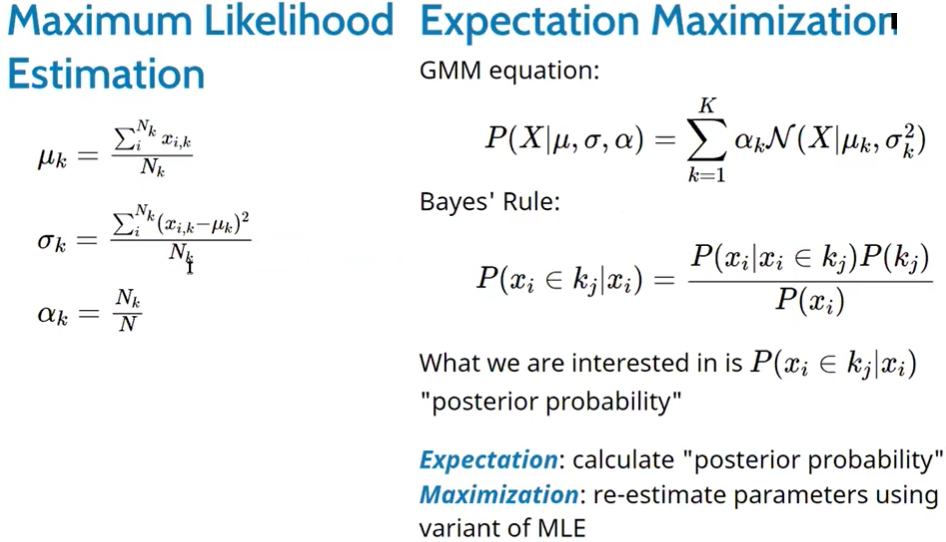
\includegraphics[scale = 0.5]{GMM_6} %width=\textwidth
\caption{\textit{GMM 6}}
\end{figure}

\begin{figure}[H]
\centering
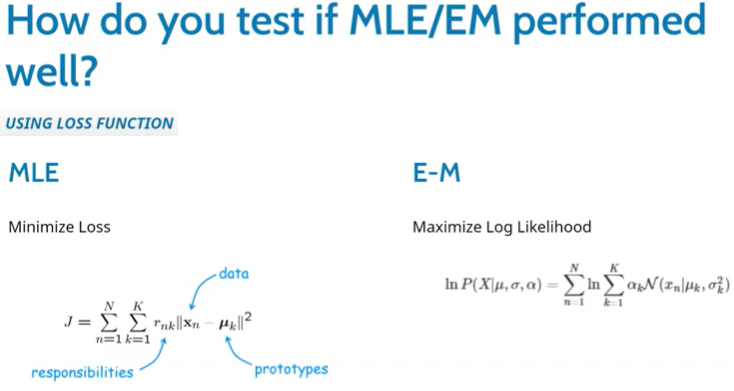
\includegraphics[scale = 0.5]{GMM_7} %width=\textwidth
\caption{\textit{GMM 7}}
\end{figure}

\subsection{Obtención de D'}

\textbf{Parámetros iniciales:}

\begin{enumerate}
\item Obtener $D$ y $D'_{0}$ con la función \textit{gen\_mat\_demanda\_alumnos}

\item Calificar $D'_{0}$ con respecto a $D$: Las calificaciones dependen de la diferencia relativa entre $D$ y $D'_{0}$. En caso de que haya un cero en la entrada correspondiente en $D$, entonces: si sobran alumnos la calificación es -1 y si faltan es 1.

\item Aplicar modelo de mezcla de normales: Obtener la distribución por materia.
\end{enumerate}

\textbf{Pasos a repetir:}

\begin{enumerate}
\item Obtener $D'_{k}$: Se corrige la materia $j$ si su calificación (por materia) está fuera del intervalo $[-20,10]$. Se corrige el número de alumnos simulados por hora, si su calificación (por grupo) está fuera del intervalo $[-10,10]$. El número de alumnos simulados se genera a partir de la distribución obtenida con el modelo de mezcla de normales.

\item Calificar $D'_{k}$ con respecto a $D$: Las calificaciones dependen de la diferencia relativa entre $D$ y $D'_{k}$. En caso de que haya un cero en la entrada correspondiente en $D$, entonces: si sobran alumnos la calificación es -1 y si faltan es 1.

\item Aplicar modelo de mezcla de normales: Obtener la distribución por materia.

\item Repetir hasta que ya no haya materias con calificación fuera de $[-20,10]$.
\end{enumerate}


\begin{figure}[H]
\centering
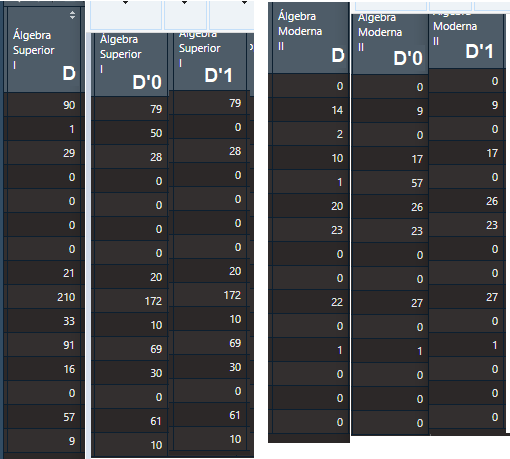
\includegraphics[scale = 1]{Ej_gmm} %width=\textwidth
\caption{\textit{Ejemplo de la obtención de D'}}
\end{figure}

